\section{Selection of Important Single Nucleotide Polymorphisms behind behavioral traits from Familial Genome Wide Association Studies data}
\label{sec:TwinSection}

\subsection{Motivation}
Genome Wide Association Studies (GWAS), where genetic variants across the full human genome are analyzed, are becoming more and more relevant in recent years for the purpose of determining which of the variants are associated behind the expression of complex traits. The advent of efficient and economical genotyping technology enables researchers to scan the genome at hundreds of thousands of Single Nucleotide Polymorphisms (SNPs), and improvements in computational speed in the past few decades have helped in feasible analysis of the huge amount of data collected in order to detect significant associations \citep{VisscherEtal12}. One major challenge in such studies is the small effects individual SNPs have: detecting which requires large sample sizes \citep{ManolioEtal09}. For quantitative behavioral traits, for example alcohol dependence, drug abuse, Anorexia and depression, this problem is amplified because of the additional noise introduced by variation due to the environment the subject grew up in. This is one of the motivations of performing GWAS on families (GWAF) instead of unrelated individuals, through which the environmental variation can be reduced: so as to require smaller samples to detect the same magnitude of SNP effect. Another major reason, of course, of performing GWAS on familial data is to detect gene-environment interactions associated with development of behavioral traits. The data analyzed in such families typically consist of trait information and genotypes of from parents and their children, who can be either identical twins, non-identical twins or adpoted.

Single-marker tests, i.e. analyzing the effect of multiple SNPs separately on the quantitative phenotype and then selecting a group of SNPs by setting suitable thresholds on the resulting $p$-values, often after correction for multiple testing, is the most commonly used method to detect SNPs associated with the phenotype being studied. Although simultaneously estimating the fixed effect of a single SNP as well as the stratified population variance covariance matrix reflecting the familial structure, and repeating this for a large number of SNPs is a computationally prohibitive task, several fast approximation methods exist in the literature that tackle this while maintaining moderately high power. The GRAMMAR method of \cite{AulchenkoEtal07} and the association test of \cite{ChenAbecasis07} are examples of this. While these two methods are able to efficiently analyze GWAF data, they assume that phenotypic similarity within families is entirely due to their genetic similarity and ignore the effect of shared environment. In GWAF data from nuclear (i.e. unrelated) families, the proportion of phenotypic variation explained by the shared environmental effects is often substantial, sometimes as high as 51\% \citep{McGueEtal13} or 74\% \citep{DeNeveEtal13}: in which case such methods shall not be able to account for this added variation. To remedy this, \cite{LiEtal11} proposed a rapid method (RFGLS) that computes $p$-values corresponding to each SNP through a rapid approximation of the single-SNP generalized least squares model taking into account genetic and environmental sources of familial similarity.

A major issue with all such methods of single-marker analysis is that they are not always effective for detecting functionally relevant SNPs or regions in the genome. A single SNP is sometimes not enough to capture the extent of association \citep{YangEtal12, Ke12}. This includes cases when there are multiple causal SNPs closely located inside a gene in high Linkage Disequilibrium (LD) with one another. The causal SNP may even not be genotyped if its variants are unlikely to be present in the sample population (e.g. the variant of the SNP rs671 responsible for low alcohol tolerance in asians is rare in caucasians), and other SNPs highly correlated with it are genotyped instead.

%Due to the weak signal of individual SNPs as well as the heavy amount of correlation among them, detecting SNPs that are actually associated with the quantitative trait being analyzed is statistically challenging. A major impediment of estimating effects of multiple SNPs \textit{while} taking into account theirIn any kind of GWAS, fitting separate models on single markers typically suffer from loss of power.
% However the dependent data structure and large sample sizes in familial GWAS data calls for usage of suitable statistical models, for example mixed effet modelling, which makes even training a single model computationally intensive. and because of this any traditional variable selection approach is infeasible in such setup.

Here we propose to tackle this through fitting mixed effect models with the behavioral trait phenotype as respone and a group of SNPs (e.g. SNPs inside a single gene) as fixed effect predictors, and selecting important SNPs through a model selection approach. Although the major impediment of applying model selection techniques in GWAS setup is the high computational cost, some fast methods have been proposed that are able to perform SNP seletion from a multi-SNP model on GWAS data from \textit{unrelated individuals} \citep{ZhangEtal14,FrommeletEtal12}. However, these methods still rely on fitting models corresponding to multiple predictor sets. This makes them unsuitable to be adapted to the GWAF setup because of the much higher computational costs associated with training multiple mixed effect models that take into account within-family correlation between individuals, as compared to models that assume independent observations.

We shall use our $e$-values framework to provide a solution to this situation. As showed in the last chapter, our variable selection technique based on $e$-values requires only fitting the `full model': which makes it suitable to be utilized here.

\subsection{The MCTFR data}
The familial GWAS dataset collected and studied by Minnesota Center for Twin and Family Research (MCTFR)\citep{LiEtal11, MillerEtal12, McGueEtal13} consists of samples from three longitudinal studies conducted by the MCTFR: (1) the Minnesota Twin Family Study (MTFS: \cite{IaconoEtal99}) that covers twins and their parent, (2) the Sibling Interaction and Behavior Study (SIBS: \cite{McGueEtal07}) that includes adopted and biological sibling pairs and their parents, and (3) the enrichment study (ES: \cite{KeyesEtal09}) that extended the MTFS by oversampling 11 year old twins who are highly likely to develop substance abuse. While 9827 individuals completed the initial assessments for participation in the study, after several steps of screening the final sample consisted of 7188 caucasian individuals clustered in 2300 nuclear families. %Here a total of 7188 Caucasian individuals, who come from $\sim 2300$ families, have been genotyped. A detailed description of the data is available at \cite{MillerEtal12}.

DNA samples collected from the subjects were analyzed using Illumina’s Human660W-Quad Array for 561,490 non-intensity SNP markers. After several data cleaning steps for quality control, 527,829 SNPs were retained. Covariates for each sample included age, sex, birth year, generation (parent or offspring), as well as two-way interactions between generation and other three covariates each. As for the quantitative phenotypes, five of them were studied in this GWAS: (1) Nicotine dependence, (2) Alcohol consumption, (3) Alcohol dependence, (4) Illegal drug usage, and (5) Behavioral disinhibition. The response variables corresponding to these phenotypes were derived from questionnaires using a hierarchical approach based on factor analysis \citep{HicksEtal11}.

A more detailed description of the data is available  in \cite{MillerEtal12}. Several studies have been performed that focus on different aspects of this dataset. \cite{LiEtal11} used RFGLS to single out causal SNPs behind the height of participants, while \cite{McGueEtal13} used the same method to study SNPs behind the development of all five indicators of behavioral disinhibition mentioned above. \cite{IronsThesis12} focused on the effect of several factors affecting alcohol use in the study population, namely the effects of polymorphisms in the ALDH2 gene and the GABA system genes, as well as the effect of early exposure to alcohols as adolescents to adult outcomes. Finally \cite{CoombesThesis16} used a bootstrap-based combination test and a sequential score test to evaluate gene-environment interactions behind phenotypic outcomes in the data.

\subsection{Statistical model}
We shall demonstrate the use of $e$-values in this context using a Linear Mixed Model (LMM) framework. We assume that the families modeled are unrelated to one another, i.e. they are nuclear pedigrees. We stick to this structure for ease of representation, although as discussed shortly, the model fitting process remains unchanged for larger pedigrees.

We assume there are a total of $m$ families, with the $i$-th pedigree containing $n_i$ individuals. Denote by $\bfy_i = (y_{i 1}, \ldots, y_{i n_i})^T $ the quantitative trait values for individuals in that pedigree, while the matrix $\bfG_i \in \BR^{ n_i \times p_s}$ containing their genotypes for a bunch of SNPs. Let $\bfC_i \in \BR^{ n_i \times p}$ denote the data on $p$ covariates for individuals in the pedigree $i$. Given these, we consider the following model.
%
\begin{align}\label{eqn:LMMeqn}
\bfY_i = \alpha + \bfG_i \bfbeta_g + \bfC_i \bfbeta_c + \bfepsilon_i
\end{align}
%
with $\alpha$ the intercept term, $\bfbeta_g$ and $\bfbeta_c$ fixed coefficient terms corresponding to the multiple SNPs and covariates, respectively, and $\bfepsilon_i \sim \cN_{n_i} (\bfZero, \bfV_i)$ the random error term. To account for the within-family dependency structure, we break up the random error variance into three independent components:
%
\begin{align}\label{eqn:partsOfV}
\bfV_i = \sigma_a^2 \bfPhi_i + \sigma_c^2 {\bf 1} {\bf 1}^T + \sigma_e^2 \bfI_{n_i}
\end{align}
%
The first part represents a within-family random effect term to account for effects of other SNPs. The matrix $\bfPhi_i$ is the relationship matrix within the $i$-th pedigree. Its $(s,t)$-th element represents two times the kinship coefficient, which is the probability that given that a random gene is drawn each from individuals $s$ and $t$ in pedigree $i$, these genes are `identical by descent', i.e. come from same common ancestor. The second part accounts for shared environmental effect within the family, while the third term finally quantifies other sources of variation unique to an individual.

Following basic probability, the kinship coefficient of a parent-child pair is 1/4, a full sibling pair or non-identical (or dizygous = DZ) twins is 1/4, and for identical (or monozygous = MZ) twins is 1/2 in a nuclear pedigree. Following this, we can construct the $\bfPhi_i$ matrices for different types of families:
%
\begin{align*}
\bfPhi_{MZ} = \begin{bmatrix}
1 & 0 & 1/2 & 1/2 \\
0 & 1 & 1/2 & 1/2 \\
1/2 & 1/2 & 1 & 1\\
1/2 & 1/2 & 1 & 1
\end{bmatrix},
\bfPhi_{DZ} = \begin{bmatrix}
1 & 0 & 1/2 & 1/2 \\
0 & 1 & 1/2 & 1/2 \\
1/2 & 1/2 & 1 & 1/2\\
1/2 & 1/2 & 1/2 & 1
\end{bmatrix},
\bfPhi_{Adopted} = \bfI_4
\end{align*}
%
for families with parents (indices 1 and 2) and MZ twins, DZ twins, or two adapted children (indices 3 and 4), respectively.

We use the R package \texttt{regress} to fit the above model with additive error structure. The package requires specifying the dependency structure of all samples in the data. For ease of representation, we only consider nuclear pedigrees with MZ twins in our simulation study and data analysis, which simplifies the overall relationship matrix $\bfPhi = \text{diag} ( \bfPhi_1, \ldots, \bfPhi_m)$ as $\bfI_m \otimes \bfPhi_{MZ}$. Note that, situations in which the pedigree structure is not nuclear can be readily handled in this situation by supplying the overall $\bfPhi$ matrix. The second overall structural component will be  $\bfI_m \otimes {\bf 1} {\bf 1}^T$. The \texttt{regress} procedure includes the third structure in \ref{eqn:partsOfV} by default.

\subsection{A conditional $e$-value}
We now take a closer look at the evaluation map distributions corresponding to reduced model coefficient estimates, in order to better detect the weak signals we are dealing with here and reduce the number of false positives. Carrying over notations from \ref{chapter:Chapter-evalue}, recall that the model formed by dropping the $j$-the index is denoted by $\cM_{-j}$, and we are going to inspect $\BD_{-j}$, the distribution of $D( \hat \bfbeta_{-j}, [\hat \bfbeta] ) $ by comparing it with $\BD :=$ distribution of $D( \hat \bfbeta, [\hat \bfbeta] ) $. Also define by $\mu(.)$ the mean operator on the corresponding distributions.

Recall from \ref{chapter:Chapter-evalue} that we approximate the above distributions and the final $e$-value through resampling. The quality of approximation depends on the variance parameter $\tau_n^2$, and as seen in the simulation section, on the type of bootstrap scheme used (moon/ gamma/ generalized). Because of the high-computational overhead of the \texttt{regress} procedure, we shall use the parametric generalized bootstrap scheme here. We would also like to emphasize that all observations in this subsection are entirely empirical and from controlled simulation setups, and further studies are warranted to theoretically characterize such behavior.

We denote by $\hat \BD_{-j} (\tau)$ and $\hat\BD (\tau)$ the approximations of $\BD_{-j}$ and $\BD$, respectively, using a generalized bootstrap scheme with standard deviation $\tau_n \equiv \tau$. According to theorem \ref{Theorem:ModelScore}, in case $\BD_{-j}$ is an inadequate model distribution, the mean of $\hat \BD_{-j} (\tau)$ goes to 0 in probability for an intermediate rate of the bootstrap standard deviation. As $\tau$ increases, all reduced model distributions approach $\hat\BD (\tau)$. However, depending on the magnitude of signals at the non-zero indices, we observe that this behavior follows two different regimes. We demonstrate this using the simulation setup we elaborate on later in the chapter. In the plots below, $h$ represents the relative magnitude of non-zero entries in the coefficient vector: for which we consider two choices, $h=5$ and $h=0.05$.

\begin{figure}
\centering
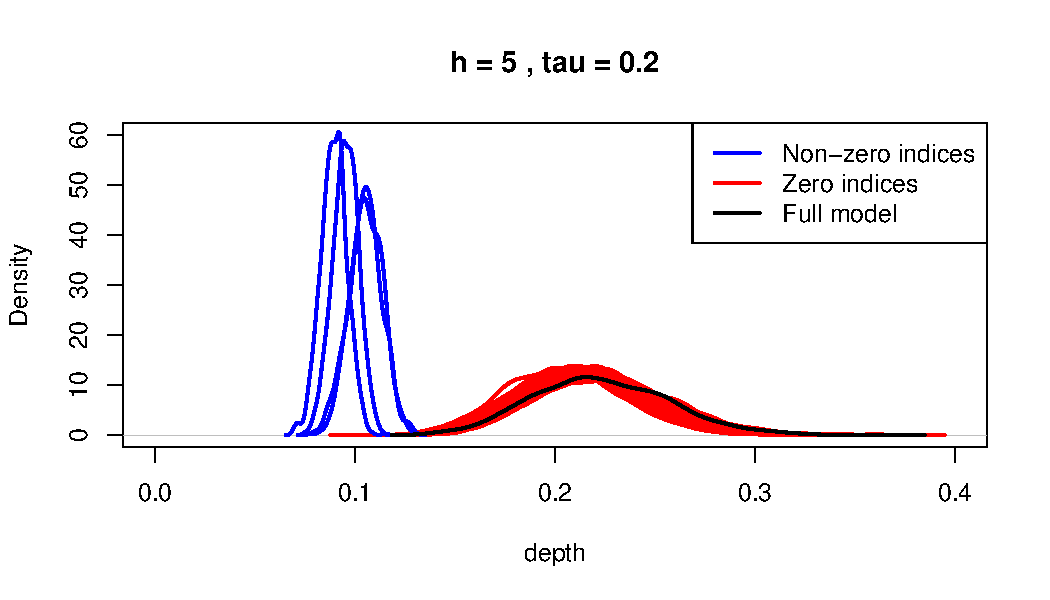
\includegraphics[height=.22\textheight]{Chapter-appli/plot_h5_tau2}\\
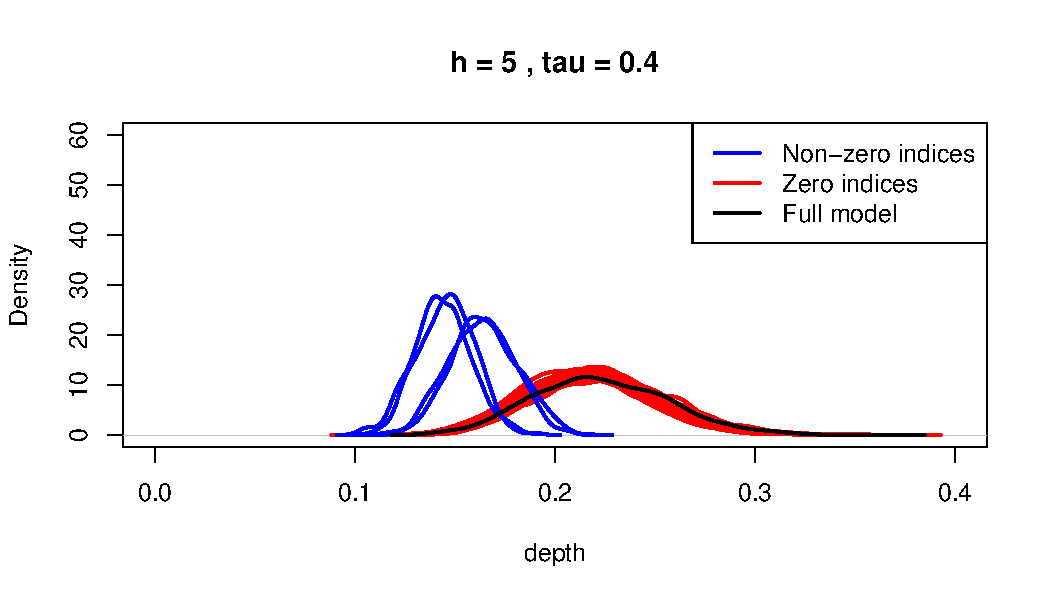
\includegraphics[height=.22\textheight]{Chapter-appli/plot_h5_tau4}\\
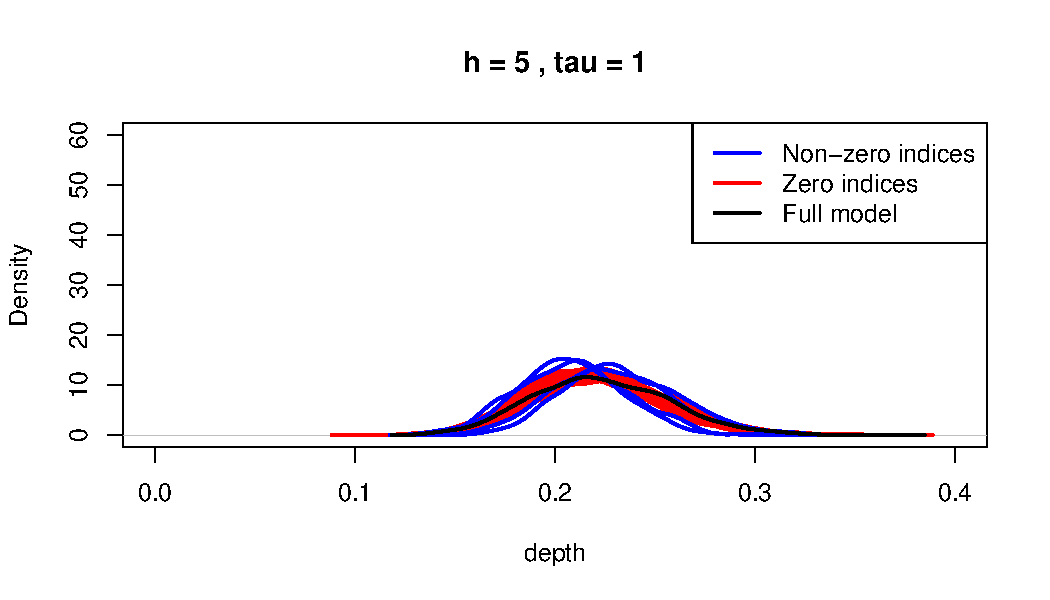
\includegraphics[height=.22\textheight]{Chapter-appli/plot_h5_tau10}\\
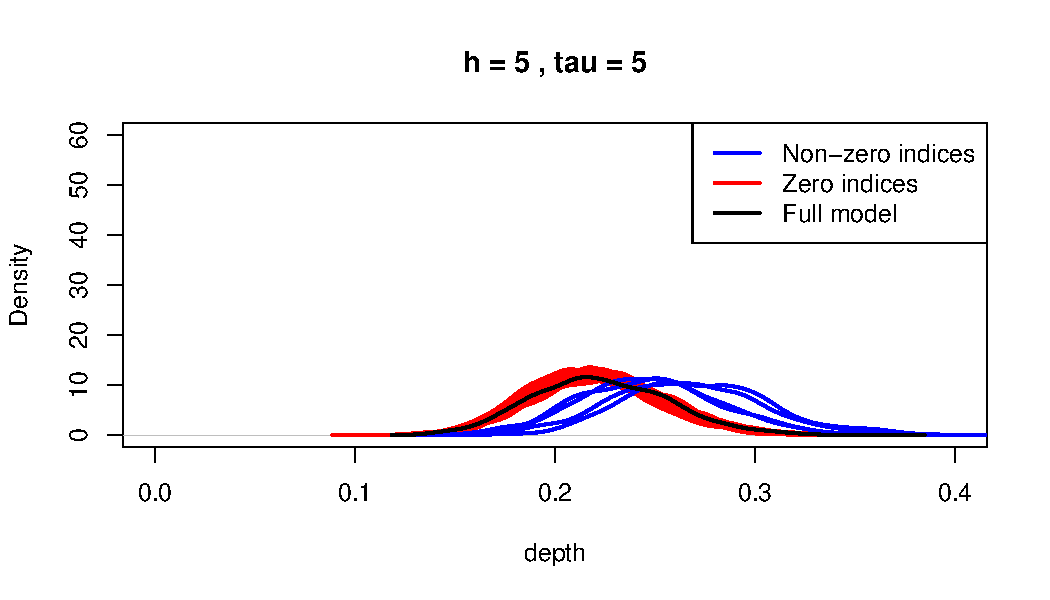
\includegraphics[height=.22\textheight]{Chapter-appli/plot_h5_tau50}
\caption{Density plots for $\hat \BD(\tau)$ and $\hat \BD_{-j}(\tau)$ for all $j$ in simulation setup, with signal parameter $h=5$ and bootstrap standard deviations $\tau = 0.2, 0.4, 1, 5$}
\label{fig:figLargeTau1}
\end{figure}

\begin{figure}
\centering
\includegraphics[height=.22\textheight]{{"Chapter-appli/plot_h0.05_tau2"}.pdf}\\
\includegraphics[height=.22\textheight]{{"Chapter-appli/plot_h0.05_tau4"}.pdf}\\
\includegraphics[height=.22\textheight]{{"Chapter-appli/plot_h0.05_tau10"}.pdf}\\
\includegraphics[height=.22\textheight]{{"Chapter-appli/plot_h0.05_tau50"}.pdf}
\caption{Density plots for $\hat \BD(\tau)$ and $\hat \BD_{-j}(\tau)$ for all $j$ in simulation setup, with signal parameter $h=0.05$ and bootstrap standard deviations $\tau = 0.2, 0.4, 1, 5$}
\label{fig:figLargeTau2}
\end{figure}

\paragraph{(a) Large signal regime ($h=5$: \ref{fig:figLargeTau1})} When $\BD_{-j}$ corresponds to an inadequate model, i.e. the $j$-th coefficient of the true parameter vector is non-zero, for small values of $\tau$ we can clearly distinguish this distribution from that of $\hat\BD (\tau)$ in their density plots. As $\tau$ increases, the inadequate model distributions seem to have more and more positive bias. However, when $j$ is a non-essential covariate, the reduced distributions are close to $\hat \BD(\tau)$ for all values of $\tau$.

\paragraph{(b) Small signal regime ($h=0.05$: \ref{fig:figLargeTau2})} When the actual signal in $\beta_j$ is weak, the inadequate reduced model distributions still approach $\hat \BD(\tau)$ as $\tau$ goes up but stabilize at the full model distribution instead of passing it for very large $\tau$ ($\tau=5$ here). However the adequate model distributions seem to exhibit a similar behavior: albeit staying to the left of inadequate model density plots in general.

This increased ambiguity of reduced model distributions for small signals make it difficult to distinguish between two types of model distributions using the mean operator, which ends up being very conservative in the second case. For this reason we consider the usage of a different summarizing function that will be able to capture the differentiate between the two types of reduced model distributions across a broader range of the signal-to-noise ratio, specifically by setting a lower detection threshold than the same operator on the full model distribution. Here we focus on a specific alternate formulation of the $e$-value that is based on a tail quantile of $\hat \BD_{-j} (\tau)$:
%
\begin{align}
e_q (\cM_{-j} | \tau) = q \text{-th quantile of } \hat \BD_{-j} (\tau)
\end{align}
%
for some fixed $q \in (0,1)$. Notice that for any $q$, the quantity $e_q (\cM_{-j} | \tau)$ is conditional on the bootstrap standard deviation parameter $\tau$.

The motivation behind this is the observation that the inadequate and adequate model distributions have different tail behaviors for intermediate values of $\tau$, and setting an appropriate upper threshold to tail probabilities for a suitable fixed quantile of these distributions with respect to $\hat \BD(\tau)$ can possibly separate out the two types of distributions. The choice of threshold potentially depends on several factors such as the value of $q$, the statistical model used, degree of sparsity of parameters in the data generating process. In the following section we shall experiment with different thresholds to illustrate this.
Also note that we still retain the main flavor of the $e$-values method, by training only the full model and then use Monte Carlo resampling to compute $e_q (\cM_{-j} | \tau)$ for all $j$ and a range of $\tau$.

\subsection{Simulation}
\label{sec:SimSection}

We now compare the performance of the above formulation of quantile $e$-values in a simulation setup. For this, consider the model in \ref{eqn:LMMeqn} with no environmental covariates. We consider familes with MZ twins and first generate the covariate matrices $\bfG_i$. We take a total of $p_g = 50$ SNPs, and to simulate correlation among SNPs in the genome generate them in correlated blocks of 6, 4 ,6, 4 and 30. We set the correlation between two SNPs inside a block at 0.7, and consider the blocks to be uncorrelated. For each parent we generate two independent vectors of length 50 with the above correlation structure, and entries within each block being 0 or 1 following Bernoulli distributions with probabilities 0.2, 0.4, 0.4, 0.25 and 0.25 (Minor Allele Frequency or MAF) for SNPs in the 5 blocks, respectively. The genotype of a person is then determined by taking the sum of these two vectors: thus entries in $\bfG_i$ can take the values 0, 1 or 2. Finally we set the common genotype of the twins by randomly choosing one allele vector from each of the parents and taking their sum.

We repeat the above process for $m=250$ families. In GWAS there are generally a small number of causal SNPs, each explaining small proportions of the overall variability in response variable. To reflect this in our simulation setup, we assume that the first entries in each of the first four blocks above are causal, and each of them explains $h/(\sigma_a^2+\sigma_c^2+\sigma_e^2) \%$ of the overall variability. The term $h$ is known as the \textit{heritability} of the corresponding SNP (and can of course vary across SNPs). The value of the non-zero coefficient in $k$-th group: $k = 1, ..., 4$, say $\beta_k$ is calculated using the formula:
%
\begin{align}
\beta_k = \sqrt{ \frac{h}{(\sigma_a^2+\sigma_c^2+\sigma_e^2). 2 \text{MAF}_k (1 - \text{MAF}_k) }}
\end{align}
%
We fix the following values for the error variance components: $\sigma_a^2 = 4, \sigma_c^2 = 1, \sigma_e^2 = 1$, and generate pedigree-wise response vectors $\bfy_1, \ldots, \bfy_{250}$ using the above setup. To consider different SNP effect sizes, we repeat the above setup for $h \in \{10, 5, 2, 1, 0 \}$, generating 1000 datasets for each value of $h$.

\subsubsection{Methods and metrics}
For this simulated data, we compare our $e$-value based approach with two other methods:

\paragraph{(1) Model selection on linear model:} Here we ignore the dependency structure within families by training linear models on the simulated data and selecting SNPs with non-zero effects by backward deletion using a modification of the BIC called mBIC2. This has been showed to give better results than single-marker analysis in GWAS for unrelated individuals \citep{FrommeletEtal12} and provides approximate False Discovery Rate (FDR) control at level 0.05 \citep{BogdanEtal11}.

\paragraph{(2) Single-marker mixed model:} We train single-SNP versions of \ref{eqn:LMMeqn} using a fast approximation of the Generalized Least Squares procedure (named Rapid Feasible Generalized Least Squares or RFGLS: \cite{LiEtal11}), obtain marginal $p$-values from corresponding $t$-tests and use the Benjamini-Hochberg (BH) procedure to select significant SNPs at FDR = $0.05$.

\vspace{1em}\noindent We compute the $e$-values by setting projection depth \citep{zuo03} as the evaluation function. With the $e$-value being the $q$-th quantile of the evaluation map distribution, we set the detection threshold value at the $t$-th multiple of $q$ for some $0 < t < 1$. This means all indices $j$ such that $q$-th quantile of the bootstrap approximation of $\hat \BD_{-j} (\tau)$ is less than the $tq$-th quantile of $\hat \BD (\tau)$ will get selected as the set of active predictors. We repeat the $e$-value procedure for different values of the bootstrap standard deviation $s \in \{ 0.3, 0.35, \ldots, 0.95, 2 \}$. Consequently, we take as the final estimated set of SNPs the SNP set $\hat \cS (\tau)$ that minimizes fixed effect prediction error (PE) on an independently generated test dataset $\{ (\bfy_{test,i}, \bfG_{test,i}), i = 1, \ldots, 250 \}$ from the same setup above:
%
\begin{align*}
& \text{PE} (\tau | q,t)  = \sum_{i=1}^{250} \sum_{j=1}^4 \left( y_{test,ij} - \bfg_{test,ij}^T \hat \bfbeta_{\hat \cS (\tau)} \right)^2; \\
& \hat \cS_0 (q,t) = \argmin_\tau \text{PE} (\tau | q,t)
\end{align*}

The metrics to evaluate each method we implement are:

\begin{enumerate}
\item True Positive (TP): proportion of causal SNPs detected;

\item True Negative (TN): proportion of non-causal SNPs undetected;

\item Relaxed True Positive (TPR): proportion of detecting any SNP in each of the 4 blocks with causal SNPs, i.e. for the selected index set $\hat \cS_0 (q,t)$,
%
$$
\text{TPR} ( \hat \cS_0 (q,t) ) = \frac{1}{4} \sum_{i=1}^4 \BI ( \text{Block } i \cap \hat \cS_0 (q,t) \neq \emptyset )
$$
%

\item Relaxed True Negative (TNR): proportion of SNPs in block 5 undetected.
\end{enumerate}

\noindent We consider the third and fourth metrics to cover situations in which the causal SNP is not detected itself, but highly correlated SNPs with the causal SNP are. This is common in GWAS. Finally, we average all the above proportions over 1000 replications, and repeat the process for $ q \in \{ 0.9, 0.5, 0.2, 0.1 \}; t \in \{ 0.8, 0.7, 0.6, 0.5 \}$.

%Although the first two heritability values are larger compared to a typical GWAS setup, we use this setup to demonstrate limitations of the existing methodology even in a vastly simplified setting.

\subsubsection{Results}
% latex table generated in R 3.3.2 by xtable 1.8-2 package
% Sun Apr 16 18:24:09 2017
% latex table generated in R 3.3.2 by xtable 1.8-2 package
% Sun Apr 16 18:24:48 2017
\begin{table}
\begin{footnotesize}
\centering
    \begin{tabular}{c|c|c|c|cccc}
    \hline
     6x   & mBIC2       & RFGLS  & \multicolumn{5}{|c}{quantile $e$-values}    \\\cline{4-8}
    Heritability    &           & +BH		 & $q$    & $t=0.8$     & $t=0.7$     & $t=0.6$     & $t=0.5$     \\ \hline
    ~    & ~         & ~         & 0.9      & 0.95/0.97 & 0.95/0.97 & 0.95/0.98 & 0.94/0.98 \\
    $h=10$ & 0.79/0.99 & 0.95/0.92 & 0.5      & 0.96/0.97 & 0.96/0.98 & 0.95/0.98 & 0.94/0.98 \\
    ~    & ~         & ~         & 0.2      & 0.96/0.94 & 0.96/0.97 & 0.95/0.97 & 0.95/0.98 \\\hline
    ~    & ~         & ~         & 0.9      & 0.72/0.95 & 0.7/0.96  & 0.69/0.96 & 0.66/0.97 \\
    $h=5$  & 0.41/0.99 & 0.62/0.97 & 0.5      & 0.78/0.94 & 0.75/0.94 & 0.72/0.95 & 0.71/0.96 \\
    ~    & ~         & ~         & 0.2      & 0.83/0.91 & 0.78/0.94 & 0.75/0.95 & 0.73/0.95 \\\hline
    ~    & ~         & ~         & 0.9      & 0.26/0.97 & 0.24/0.97 & 0.23/0.98 & 0.21/0.98 \\
    $h=2$  & 0.11/0.99 & 0.14/0.99 & 0.5      & 0.34/0.95 & 0.28/0.96 & 0.27/0.97 & 0.26/0.97 \\
    ~    & ~         & ~         & 0.2      & 0.46/0.91 & 0.34/0.95 & 0.3/0.96  & 0.27/0.96 \\\hline
    ~    & ~         & ~         & 0.9      & 0.12/0.98 & 0.1/0.98  & 0.09/0.99 & 0.08/0.99 \\
    $h=1$  & 0.05/0.99 & 0.04/0.99    & 0.5      & 0.16/0.96 & 0.13/0.97 & 0.12/0.97 & 0.11/0.98 \\
    ~    & ~         & ~         & 0.2      & 0.25/0.93 & 0.16/0.96 & 0.13/0.97 & 0.13/0.97 \\\hline
    ~    & ~         & ~         & 0.9      & --/0.99 & --/0.99 & --/0.99 & --/0.99    \\
    $h=0$  & --/0.99 & --/0.99       & 0.5      & --/0.98 & --/0.98 & --/0.99 & --/0.99 \\
    ~    & ~         & ~         & 0.2      & --/0.94 & --/0.98 & --/0.98 & --/0.99 \\\hline
    \end{tabular}
    \caption{Average True Positive (TP) and True Negative (TN) proportions over 1000 replications for all three methods}
    \label{table:SNPSimTable0}
\end{footnotesize}
\end{table}

%% latex table generated in R 3.3.2 by xtable 1.8-2 package
%% Sun Apr 16 18:24:09 2017
%% latex table generated in R 3.3.2 by xtable 1.8-2 package
%% Sun Apr 16 18:24:48 2017
%\begin{table}
%\begin{footnotesize}
%\centering
%    \begin{tabular}{c|c|c|c|cccc}
%    \hline
%    6x    & mBIC2       & RFGLS  & \multicolumn{5}{|c}{quantile $e$-values}    \\\cline{4-8}
%    Heritability    &           & +BH		 & $q$    & $t=0.8$     & $t=0.7$     & $t=0.6$     & $t=0.5$     \\ \hline
%     ~    & 0.27/0.98 & 0.96/0.99 & 0.9      & 0.95/0.97 & 0.95/0.97 & 0.94/0.97 & 0.94/0.98 \\
%    ~    & ~         & ~         & 0.5      & 0.98/0.96 & 0.97/0.97 & 0.96/0.97 & 0.96/0.97 \\
%    h=10 & ~         & ~         & 0.2      & 0.99/0.9  & 0.97/0.96 & 0.97/0.97 & 0.96/0.97 \\
%    ~    & ~         & ~         & 0.1      & 0.99/0.83 & 0.98/0.93 & 0.97/0.96 & 0.96/0.97 \\
%    ~    & ~         & ~         & 0.05     & 0.99/0.74 & 0.98/0.88 & 0.97/0.94 & 0.97/0.96 \\ \hline
%    ~    & 0.16/0.98 & 0.63/0.99 & 0.9      & 0.74/0.95 & 0.73/0.95 & 0.71/0.96 & 0.69/0.97 \\
%    ~    & ~         & ~         & 0.5      & 0.83/0.93 & 0.78/0.94 & 0.76/0.95 & 0.75/0.95 \\
%    h=5  & ~         & ~         & 0.2      & 0.9/0.87  & 0.83/0.93 & 0.79/0.94 & 0.76/0.95 \\
%    ~    & ~         & ~         & 0.1      & 0.93/0.79 & 0.86/0.9  & 0.81/0.93 & 0.78/0.94 \\
%    ~    & ~         & ~         & 0.05     & 0.95/0.72 & 0.88/0.86 & 0.83/0.91 & 0.79/0.93 \\ \hline
%    ~    & 0.09/0.98 & 0.16/1    & 0.9      & 0.32/0.96 & 0.29/0.97 & 0.27/0.97 & 0.24/0.98 \\
%    ~    & ~         & ~         & 0.5      & 0.45/0.94 & 0.34/0.96 & 0.32/0.96 & 0.3/0.97  \\
%    h=2  & ~         & ~         & 0.2      & 0.66/0.86 & 0.47/0.93 & 0.38/0.95 & 0.33/0.96 \\
%    ~    & ~         & ~         & 0.1      & 0.77/0.79 & 0.57/0.9  & 0.43/0.94 & 0.37/0.95 \\
%    ~    & ~         & ~         & 0.05     & 0.82/0.71 & 0.64/0.85 & 0.5/0.92  & 0.41/0.94 \\ \hline
%    ~    & 0.07/0.98 & 0.05/1    & 0.9      & 0.16/0.97 & 0.14/0.98 & 0.13/0.98 & 0.11/0.99 \\
%    ~    & ~         & ~         & 0.5      & 0.26/0.95 & 0.18/0.97 & 0.17/0.97 & 0.15/0.98 \\
%    h=1  & ~         & ~         & 0.2      & 0.5/0.88  & 0.28/0.94 & 0.2/0.96  & 0.17/0.97 \\
%    ~    & ~         & ~         & 0.1      & 0.65/0.79 & 0.4/0.91  & 0.26/0.95 & 0.2/0.97  \\
%    ~    & ~         & ~         & 0.05     & 0.73/0.71 & 0.51/0.86 & 0.35/0.92 & 0.24/0.95 \\ \hline
%    ~    & 0.05/0.98 & 0.01/1    & 0.9      & 0.04/0.98 & 0.04/0.99 & 0.03/0.99 & 0.03/0.99 \\
%    ~    & ~         & ~         & 0.5      & 0.1/0.97  & 0.05/0.98 & 0.04/0.98 & 0.04/0.98 \\
%    h=0  & ~         & ~         & 0.2      & 0.32/0.89 & 0.1/0.96  & 0.06/0.98 & 0.05/0.98 \\
%    ~    & ~         & ~         & 0.1      & 0.5/0.82  & 0.22/0.93 & 0.1/0.97  & 0.06/0.98 \\
%    ~    & ~         & ~         & 0.05     & 0.64/0.73 & 0.37/0.87 & 0.2/0.94  & 0.09/0.97 \\ \hline
%    \end{tabular}
%    \caption{Average Relaxed True Positive (TPR) and Relaxed True Negative (TNR) proportions over 1000 replications for all three methods}
%    \label{table:SNPSimTable1}
%\end{footnotesize}
%\end{table}
\begin{table}
\begin{footnotesize}
\centering
    \begin{tabular}{c|c|c|c|cccc}
    \hline
    6x    & mBIC2       & RFGLS  & \multicolumn{5}{|c}{quantile $e$-values}    \\\cline{4-8}
    Heritability    &           & +BH		 & $q$    & $t=0.8$     & $t=0.7$     & $t=0.6$     & $t=0.5$     \\ \hline
    ~    & ~         & ~         & 0.9      & 0.96/0.97 & 0.96/0.97 & 0.95/0.98 & 0.94/0.98 \\
    $h=10$ & 0.84/0.99 & 0.96/0.99 & 0.5      & 0.96/0.97 & 0.96/0.97 & 0.95/0.98 & 0.95/0.98 \\
    ~    & ~         & ~         & 0.2      & 0.97/0.95 & 0.96/0.97 & 0.96/0.97 & 0.95/0.98 \\\hline
    ~    & ~         & ~         & 0.9      & 0.73/0.95 & 0.71/0.95 & 0.7/0.96  & 0.67/0.97 \\
    $h=5$  & 0.48/0.99 & 0.64/0.99 & 0.5      & 0.79/0.93 & 0.76/0.94 & 0.73/0.95 & 0.72/0.95 \\
    ~    & ~         & ~         & 0.2      & 0.85/0.91 & 0.79/0.93 & 0.76/0.94 & 0.74/0.95 \\\hline
    ~    & ~         & ~         & 0.9      & 0.29/0.96 & 0.27/0.97 & 0.25/0.98 & 0.23/0.98 \\
    $h=2$  & 0.16/0.99 & 0.16/0.99    & 0.5      & 0.37/0.95 & 0.31/0.96 & 0.3/0.96  & 0.29/0.97 \\
    ~    & ~         & ~         & 0.2      & 0.53/0.91 & 0.38/0.95 & 0.33/0.95 & 0.3/0.96  \\\hline
    ~    & ~         & ~         & 0.9      & 0.15/0.97 & 0.13/0.98 & 0.12/0.98 & 0.1/0.99  \\
    $h=1$  & 0.08/0.99 & 0.05/0.99    & 0.5      & 0.2/0.96  & 0.17/0.97 & 0.15/0.97 & 0.13/0.98 \\
    ~    & ~         & ~         & 0.2      & 0.35/0.93 & 0.21/0.96 & 0.17/0.97 & 0.16/0.97 \\\hline
    ~    & ~         & ~         & 0.9      & --/0.97 & --/0.98 & --/0.98 & --/0.99 \\
    $h=0$  & --/0.98 & --/0.99    & 0.5      & --/0.95 & --/0.97 & --/0.97 & --/0.98 \\
    ~    & ~         & ~         & 0.2      & --/0.90 & --/0.95 & --/0.97 & --/0.97 \\\hline
    \end{tabular}
    \caption{Average Relaxed True Positive (TPR) and Relaxed True Negative (TNR) proportions over 1000 replications for all three methods}
    \label{table:SNPSimTable1}
\end{footnotesize}
\end{table}

We present the simulation results in \ref{table:SNPSimTable0} and \ref{table:SNPSimTable1}. Applying BIC on linear models performs poorly compared RFGLS and then correction for multiple testing on marginal LMMs for all heritability values: possibly because the linear models are trained on a smaller amount of data and ignore the variation due to shared environment in the parents.

Our proposed $e$-values work better than the two methods for detecting true signals across different values of $h$: the average TP rate going down slowly than other methods across the majority of choices for $(q,t)$. Both mBIC2 and RFGLS+BH have very high true negative detection rates, which is matched by our method for higher values of $q$. Since all reduced model distributions reside on the left of the full model distribution, we expect the variable selection process to turn more conservative at higher values of $t$.This effect is more noticeable for lower $q$. This indicates that the right tails of evaluation map distributions are more useful for this purpose. Finally for $h=0$, we report only TN or TNR values since no signals should ideally be detected: in terms of this a value of $q=0.9$ or $q=0.5$ leads to the same TN and TNR performance as RFGLS+BH for all choices of $t$. Finally, TPR performances for all methods are better than the corresponding TPTN performances. However, for mBIC2 this seems to be due to detecting SNPs in the first four blocks by chance since for $h=0$ its TNR is less than TN.

Considering that when analyzing a large number of SNPs false positives need to be minimized, setting $q=0.9, t=0.5$ is a safe choice choice for $e$-values in this simulation setup. Note here that the previous model selection algorithm using $e$-values depended on comparing the mean of the evaluation map distribution $\BD_{-j}$ with that of $\BD$. Compared to that here we end up comparing a tail quantile of $\BD$, and set the detection threshold at a smaller value than the same quantile of $\BD$.

\subsection{Analysis of the Minnesota Twin Studies data}
We now apply the above technique on genes from a familial GWAS dataset collected and studied by Minnesota Center for Twin and Family Research \citep{MillerEtal12,McGueEtal13,LiEtal11}. Here a total of 7188 Caucasian individuals, who come from $\sim 2300$ families, have been genotyped. A detailed description of the data is available at \cite{MillerEtal12}.

In total, five quantitative phenotypes were studied in this GWAS: (1) Nicotine dependence, (2) Alcohol consumption, (3) Alcohol dependence, (4) Illegal drug usage, and (5) Behavioral disinhibition. The response variables corresponding to these phenotypes were derived from questionnaires using a hierarchical approach based on factor analysis \citep{HicksEtal11}. SNP genotype data were collected from the sample using Illumina’s Human660W-Quad Array, and 529828 SNPs were retained in the dataset after a screening for quality control.

We assume a nuclear pedigree structure, and for simplicity only analyze pedigrees with MZ twins only. After adjusting for missing data, here we have 682 such 4-member families. For the response variable, we look at the effect of genetic factors behind alcohol consumption, which has previously been found to be highly heritable in this dataset \citep{McGueEtal13}. As a first pass we decide to analyze SNPs inside some of the most-studied genes with respect to alcohol abuse: GABRA2, ADH1B, ADH1C, SLC6A3, SLC6A4, OPRM1, CYP2E1, DRD2, ALDH2, and COMT \citep{CoombesThesis16} through separate gene-level models. The ADH genes did not contain many SNPs individually, so we decided to club all existing ADH genes (ADH1-ADH7) together in our analysis.

For each gene, We train the LMM in \ref{eqn:LMMeqn} on 75\% of randomly selected families, perform our conditional $e$-values procedure for $\tau = 0.2, 0.4, \ldots, 2.8, 3$; and select the predictor set $\hat \cS_0 (\tau) $ that minimizes fixed effect prediction error on the data from the other 25\% of families. To enforce a stricter control on which SNPs get selected, we use $q=0.9$ and $t=0.5$ here based on results in the simulation setup, and use projection depth as the evalution function.

% latex table generated in R 3.3.2 by xtable 1.8-2 package
% Tue Apr 18 15:37:10 2017
\begin{table}[t]
\begin{footnotesize}
\centering
\begin{tabular}{c|c|p{4in}}
    \hline
    Gene   & Total/detected & Non-zero SNPs ordered                                                                                                                                                                                                                                                                                                             \\
    ~      & SNP            & per position in genome \\  \hline
GABRA2 &  11/5 & rs572227(-), rs534459(+), rs502038(-), rs1808851(+), rs279856(-) \\ \hline
  ADH &  21/5 & rs17027523(-), rs13103626(+), rs10516430(+), rs12503056(+), rs2004316(-) \\ \hline
  SLC6A3 &  18/4 & rs2042449(+), rs464049(-), rs460700(-), rs460000(+) \\ \hline
  SLC6A4 &   5/0 & None \\ \hline
  OPRM1 &  46/29 & rs9371718(-), rs1937600(+), rs9397637(+), rs12662873(-), rs1316368(+), rs1937587(-), rs6921403(-), rs1937580(+), rs1937645(+), rs1892361(-), rs1937633(+), rs1937631(-), rs12527197(-), rs1892360(-), rs1892356(+), rs1937619(-), rs1332849(-), rs9371749(+), rs9285539(+), rs9322439(-), rs11752884(+), rs4870241(-), rs689219(-), rs9371761(+), rs12199858(+), rs9371762(-), rs612450(+), rs9384159(+), rs6938958(-) \\ \hline
  CYP2E1 &   9/5 & rs9419702(-), rs9419624(+), rs7906770(-), rs9419569(+), rs9419629(+) \\ \hline
  DRD2 &  17/0 & None\\ \hline
  ALDH2 &   5/5 & rs7398343(+), rs7297186(+), rs3803167(+), rs10219736(-), rs3742004(-) \\ \hline
  COMT &  15/9 & rs4646312(-), rs165656(-), rs165722(+), rs2239393(-), rs4680(+), rs174699(-), rs165728(+), rs5993891(+), rs2239395(-) \\  \hline
\end{tabular}
\caption{Table of analyzed genes and detected SNPs in them. Positive/ negative sign indicates type of association found.}
\label{table:genetable}
\end{footnotesize}
\end{table}

We show the results of our gene-specific analyses in \ref{fig:geneplot1}, \ref{fig:geneplot2} and \ref{fig:geneplot3}. The exon locations are obtained from annotation data extracted from the UCSC Genome Browser database \citep{UCSCdata}. Also \ref{table:genetable} summarizes the selected SNPs for each gene. In general, SNPs tend to get selected in groups with neighboring SNPs, which suggests high Linkage Disequilibrium (LD). Also most of the selected SNPs either overlap or in close proximity to the coding regions of genes, i.e. exons, which underline their functional relevance.

\begin{figure}
\begin{center}

\begin{tabular}{c}
		\includegraphics[height=.33\textwidth]{{"Chapter-appli/plotGABRA2"}.pdf}\\
		(a)\\
		\includegraphics[height=.33\textwidth]{{"Chapter-appli/plotADH"}.pdf} \\
		(b)\\	
		\includegraphics[height=.33\textwidth]{{"Chapter-appli/plotSLC6A3"}.pdf}\\
		(c)\\	
\end{tabular}

\caption{Plot of $e$-values for genes analyzed: (a) GABRA2, (b) ADH1 to ADH7, (c) SLC6A3}
\label{fig:geneplot1}

\end{center}
\end{figure}

\begin{figure}
\begin{center}

\begin{tabular}{c}
		\includegraphics[height=.33\textwidth]{{"Chapter-appli/plotSLC6A4"}.pdf}\\
		(d)\\
		\includegraphics[height=.33\textwidth]{{"Chapter-appli/plotOPRM1"}.pdf} \\
		(e)\\	
		\includegraphics[height=.33\textwidth]{{"Chapter-appli/plotCYP2E1"}.pdf}\\
		(f)\\	
\end{tabular}

\caption{Plot of $e$-values for genes analyzed: (d) SLC6A4, (e) OPRM1, (f) CYP2E1}
\label{fig:geneplot2}

\end{center}
\end{figure}

\begin{figure}
\begin{center}

\begin{tabular}{c}
		\includegraphics[height=.33\textwidth]{{"Chapter-appli/plotDRD2"}.pdf}\\
		(g)\\
		\includegraphics[height=.33\textwidth]{{"Chapter-appli/plotALDH2"}.pdf} \\
		(h)\\	
		\includegraphics[height=.33\textwidth]{{"Chapter-appli/plotCOMT"}.pdf}\\
		(i)\\	
\end{tabular}

\caption{Plot of $e$-values for genes analyzed: (g) DRD2, (h) ALDH2, (i) COMT}
\label{fig:geneplot3}

\end{center}
\end{figure}

Finally, below are some gene-specific observations:

\paragraph{GABRA2:} As seen in the plots, the first two SNPs detected are close to two separate exons. The 4th and 5th detected SNPs, rs1808851 and rs279856, are at perfect LD with rs279858 in the larger 7188-individual dataset \citep{IronsThesis12}. This SNP had not been genotyped in our sample, but is the marker in GABRA2 most frequently associated in the literature with alcohol abuse \citep{CuiEtal12}. Interestingly, a single SNP RFGLS analysis of the same twin studies data that used Bonferroni correction on marginal $p$-values to detect SNPs had missed these SNPs \citep{IronsThesis12}. This highlights the advantage of our approach.

\paragraph{ADH genes:} Multiple studies have associated rs1229984 in the ADH1B gene (position 99318162 of chromosome 4) with alcohol dependence (\url{https://www.snpedia.com/index.php/Rs1229984}), which as seen in the plot of ADH2 is close to an exon region. Our data does not contain this marker, but detects rs13103626 and rs10516430 at positions 99317251 and 99337881 respectively. The SNP rs17027523 is interesting: they reside in the uncharacterized long non-coding RNA gene LOC100507053. One previous study \citep{GelernterEtal14, XuEtal15} found significant associations for 5 SNPs in this gene with alcohol consumption for African American population through single-SNP analysis on non-familial GWAS data. Notably, their analysis found a much stronger evidence of the association in African-American part of the sample than the European American part, while our findings are entirely from a Caucasian sample.

\paragraph{SLC6A3:} Our analysis does not detect rs27072, which has been associated with alcohol withdrawal symptoms (\url{https://www.snpedia.com/index.php/Rs27072}). Two of the four neighboring SNPs we detect are in intron regions, while the other two very close to exons.

\paragraph{OPRM1:} The minor allele of the SNP rs1799971 (chr 6, position 154039662) has been associated with stronger alcohol cravings (\url{https://www.snpedia.com/index.php/Rs1799971}). We detect rs12662873 that resides within 1 kb of this SNP. There are 28 more SNPs detected by our procedure, which seem to reside in 3 clusters.

\paragraph{CYP2E1:} Five of the 9 SNPs studied are detected through our analysis. Four of them are within 10 kb of one another (base pairs 133534822 to 133543210 in chr 10). Although CYP2E1 produces one of the three major enzymes required in alcohol metabolism, effect of SNPs in this gene on alcohol dependence is sparse. In the analysis of \cite{LindEtal12} rs4646976 at 133534223 position was most associated with a measure of breath alcohol concentration: this is within our detected region. This study had also detected rs4838767 in the promoter region of CYP2E1 (position 133520114) associated with multiple alcohol consumption measures, but we did not detect the closest SNP to this as having non-zero effect on our response.

\paragraph{ALDH2:} All 5 SNPs we study are close to exons, and get picked up by the $e$-value procedure. While all five are at a lesser base pair position than the well-known SNP rs671 ({\url{https://www.snpedia.com/index.php/Rs671}, position 111803962), one of the SNPs we analyze (rs3742004) is within 5 kb of this SNP.

\paragraph{COMT:} The SNP rs4680 has long been associated with schizophrenia and substance abuse, including alcoholism. We detect this SNP with an $e$-value of 0.144, as well as 8 other SNPs. Interestingly, a previous case-control study \citep{VoiseyEtal11} associated rs4680 and rs165774 with alcohol dependence through a SNP-wise chi-squared test, and had these two SNPs in high LD in their study population. Compared to this, in our simultaneous model of all COMT polymorphisms, rs165774 is one of the two SNPs with very high $e$-value.

\paragraph{SLCA6A4 and DRD2:} Our analysis did not detect any of the SNPs in these genes having non-zero effect on alcohol consumption. Variants of these two genes have known interaction effects behind alcohol withdrawal-induced seizure \citep{KarpyakEtal10} and bipolar disorder \citep{WangEtal14}. For this reason we also ran the $e$-values procedure on the combined set of SNPs from these genes, but did not detect any signal there as well for our sample.
 
%We detected two SNPs, rs10736470 and rs10750025, within 5 kb of one another. A previous case-control study identified three SNPs at high LD associated with alcoholism in Indian population: rs1116313, TaqID or rs1800498, and rs2734835. The first two of these are in between the two SNPs we detect.


\subsection{Future work: incorporating group selection for GWAS}
To expand the above approach to the full GWAS data, we need to incorporate strategies for dealing with the hierarchical structure of SNPs: there are a large number of genes in the human genome, and each of them contains a number of SNPs. Since our method requires the number of predictors to be less than number of sample size, it is plausible to start with an initial screening step to eliminate genes that are evident not relevant. Methods like the grouped Sure Independent Screening \citep{LiZhongZhu12} and min-P test \citep{WestfallYoungBook93} will be relevant here. Following this, in a multi-gene predictor set, there are several possible strategies to select important genes \textit{and} important SNPs in them:

\begin{enumerate}
\item \textbf{Two-step $e$-values:} First construct multi-SNP models for each gene, trained on SNP data inside that gene and a common behavioral trait response and select SNPs in each model using $e$-values. Now train a modle using selected SNPs from all genes, and run group selection procedure in this model using $e$-values. This means dropping \textit{groups} of predictors from the full model and checking the reduced model $e$-values. The one-step $e$-values method outlined in \ref{chapter:evalue-chapter} will work here because of the same logic, and setting the groups as the collection of SNPs corresponding to a gene should be able to achieve our objective here.

\item \textbf{SNP-level $e$-values only:} First select important genes using an aggregation method of SNP-trait associations (e.g. \cite{LamparterEtal16}) and run $e$-value based SNP selection on the set of SNPs within these genes.

\item \textbf{Gene-level $e$-values only:} Train separate models for each gene (after initial screening), select SNPs within those models using a fast screening method (e.g. RFGLS) and run group-level or SNP-level $e$-value selection in that full set of SNPs.
\end{enumerate}

We plan to study merits and demerits of these strategies and the computational issues associated with them in detail through synthetic studies as well as in the GWAS data from MCTFR.
